\section{Non-Faradic processes and Electrical Double Layer}

So far we have described the evolution of the kinetics inside the solution inside a Faradic regime, still the system needs first to traverse a non-Faradic one where the double layer near the electrode gets created. Such a double layer is important to take into account inside experimental application since its presence can be seen as the adding of a condensator with capacity $C_{dl}$ inside the circuit that the cell form, generating an \textbf{equivalent circuit} (EQ). Therefore, what we aim to do is to model such a generation to find out an equation for $C_{dl}$, and to do this we are going to quickly describe three different type of models with increasing degrees of complexity:
\begin{itemize}[align=left, leftmargin=*]
    \item[\textbf{Helmholtz theory}.] Assume the layer as a parallel plate capacitor with a constant surface density of charge proportional to the excess charge on the metal;
    \item[\textbf{Gouy-Chapman model}.] Still a rigid charge surface is present, but gets screened by a cloud of oppositely charged ions in the solution;
    \item[\textbf{Stern model}.] Combination of the two models having one or the other depending on the distance from the surface.
\end{itemize}
\begin{figure}[t]
    \centering
    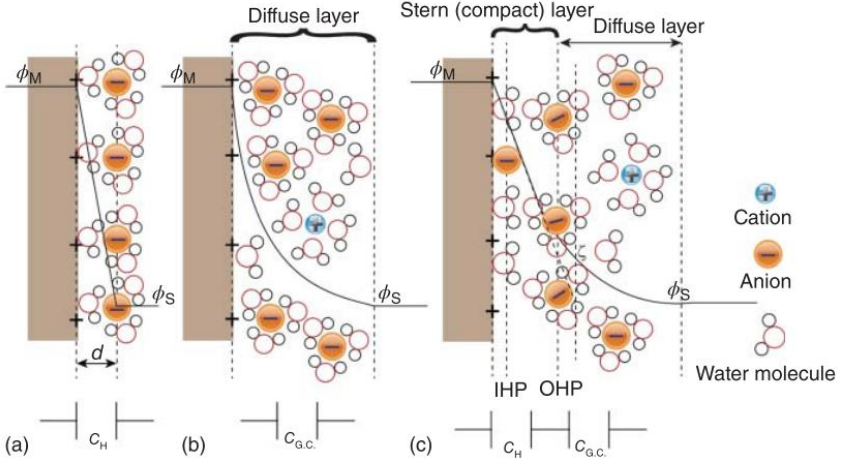
\includegraphics[width=0.8\textwidth]{Immagini/DoubleLayer.png}
    \caption{
        Graphical representation of the three models for the double layer, showing also how the potential changes inside it in the three cases.
    }
    \label{fig:DoubleLayer}
\end{figure}

\subsection{Helmholtz theory}

Inside such a simple model, which can be seen graphically in \figref{fig:DoubleLayer}, the capacity can be evaluated really easily since we know how the excess charge density on the metal is proportional to the external field $E$, having so that also the surface charge $\sigma$ on the capacitor has the same property. In this way we can write down the capacity in the following way
\begin{equation}
    C_{dl} = \pdv{\sigma}{E} = \frac{\epsilon_o\epsilon_r}{d},
\end{equation}
where $\epsilon_i$ is the dielectric constant of the specie and $d$ the width of the layer, called \textbf{Helmholtz layer}. Such a model is really simple, but posses also a lot of problems in general: predicts a \textbf{linear potential drop}, since the potential inside a capacitor is proportional to position, the \textbf{capacity not dependent on bias or charge}, and therefore also independent on concentration of electrolyte, and \textbf{overestimate the capacity}, with general values of \SI{340}{\micro\farad} versus real values of \SI{16}{\micro\farad}.

Such complication may let the reader think that this is a useless model but is rather not. In particular, if we have large potentials we effectivelly have the $C_{dl}$ has a really low dependence on potential and charge variations, leaving the model as a good simple choice that can be adopted.

\subsection{Gouy-Chapman diffuse double layer}

The concentration of the oppositely charged ions ($q^S$) decreasing with distance from the surface since they are acted upon by two forces: electrostatic attraction by $q^M$, and random thermal motion. Inside such a situation a thermodynamic study of the system can be done to see how the equilibrium distribution of the ions can be expressed in terms of potential using Boltzmann statistic that takes the following form
\begin{equation}
    C_i(x) = C_{i,b}\exp\left( -\frac{z_iF}{RT}\phi_x \right),
\end{equation}
where $\phi_i$ is the potential at distance $x$ from the surface, which we can see in \figref{fig:DoubleLayer} has a rapid decay on a longer space respect to the Helmholtz theory due to the screening given by the opposite ions diffusing near the layer. That can be evaluated thanks to the Poisson equation that can be integrated by finding a form for the charge density, which can be done in the following way
\begin{align}
    &\pdv[2]{\phi}{x} = -\frac{\rho}{\epsilon_r\epsilon_0}, &\rho(x) = F\sum_i z_iC_i(x).
\end{align}
Using the previous relation for $C_i$ and setting some boundaries conditions, such as $\phi(d) = \phi_S$ and $\phi(0) = \phi_M$, that equation can be numerically integrated to find out the wanted form of the potential. Nevertheless, it's also possible to obtain an analytic result for the charge density at the interface of the metal thanks to Gauss theorem as follows
\begin{align}
    &q^M = -\epsilon_r\epsilon_0\left( \pdv{\phi}{x} \right)_{x=0} = \sqrt{8RT\epsilon_r\epsilon_0 C_b}\sinh\left( \frac{\abs{z}F}{2RT} \phi_0\right),
\end{align}
where $\phi_0$ is referring to the potential at the surface. Now, we have the surface density as a function of the potential, meaning that we can write down a form for the capacity simply taking the derivative
\begin{equation}
    C_{G.C.} = \pdv{q^M}{\phi_0} = \abs{z}F\sqrt{\frac{\epsilon_r\epsilon_0}{RT}C_b}\cosh\left( \frac{\abs{z}F}{RT} \phi_0 \right),
\end{equation}
which is function that shows a minimum for the case where $\phi_0 = \phi_S$ that, for reasons, is equal to the situation where $q^M = 0$. That point is called \textbf{potential of zero charge} (PZC) and it's value is
\begin{equation}
    C_{G.C.}(PZC) = \abs{z}F\sqrt{\frac{\epsilon_r\epsilon_0}{RT}C_b}.
\end{equation}
This is obviously a better model since is able to predict how the capacity depends on the potential applied, but still has some problems: \textbf{High concentration} range not well-predicted, where ion-ion interactions become important and cannot be neglected, \textbf{$\epsilon_r$ constant}, while it is strongly changing in the near proximity of the electrode surface, and \textbf{ions are treated as point charges} neglecting volume and approximating the charge at the surface. 

\subsection{Stern model}

The idea of this model is to combine the two seen before by assuming that two layers are present inside the system basically: a first one composed by the electrode and the \textbf{Inner Helmoltz Plane} (IHP), where solvent and ions are specifically adsorbed to the electrode, then another between IHP and an \textbf{Outer Helmholtz Plane} (OHP), where the nearest solvated ions are non-specifically absorbed interacting via electrostatic forces. Along with such division the model assumes also that after the OHP starts the \textbf{Diffuse Layer} forming the part where the concentration is dropping exponentially with the distance as in the previous model. In this situation we can model the capacity of the double layer as the one of a system with two capacitors in series generating
\begin{equation}
    \frac{1}{C_{dl}} = \frac{1}{C_H} + \frac{1}{C_{G.C.}},
\end{equation}
basically combining the good parts of both models. Still, we have some problems with such an estimation: The solvent is also acting as a dielectric, partially shielding the charges and modifying the Helmholtz layer thickness, which we are not counting, The surface of the electrode is also hydrated to some extent, that I don't know what it means, and the degree of hydration is different between ions, still no idea. Seems that the point is that $C_{dl}$ experimentally depends on the concentration of the electrolyte and this model is not able to capture that, but I'm not sure.

\subsection{Evaluating the capacity}

To evaluate the capacity we can do a lot of things, first we always need to take into account that when we evaluate quantities inside a cell we always need to use a reference electrode to study the one we are interested in. Such electrode will so generate another interface to take into account, but usually the capacity of such electrode interface is much higher and in series respect the one of the double layer, so that the total equivalent capacity inside the equivalent circuit is $C_T \approx C_{dl}$. Taken that into account we have that the system we are dealing with is simply an RC circuit, since we have the intrinsic resistance of the solution, $R_S$, and the capacity of the double layer at work. Therefore, we can apply the known results for the current inside such a circuit to describe how the current flows inside it
\begin{equation}
    i = \frac{E}{R_S} e^{-\frac{t}{R_SC_{dl}}}.
\end{equation}
That is the solution for a constant potential, and shows how at the start a current is present, but is lowered quickly in time reaching the non-Faradic regime as expected where no current is present in the circuit, and after the double layer is charged the Faradic current, if present, can start flowing. Already here the data can be fitted with this result in order to obtain the value of $C_{dl}$, but we can do better by using a potential that vary in time as $E = \nu t$, so that the solution to the circuit becomes
\begin{equation}
    i = \nu C_{dl} \left[ 1 - e^{-\frac{t}{R_SC_{dl}}} \right],
\end{equation}
in this way we only need to evaluate the current when the system has reached the regime having a much more accurate measure.

Now, in a simple case one would assume that this behavior will not affect the current in the non-Faradic region, but that is not true. In particular, if we have a potential sweep the capacitve current is present also in the Faradic region having that the total one is $i = i_F + i_c$, but also the potential inside the solution will be changed by the drop due to the double layer which will influence both transition rate $k$ and exchange current $i_0$ in a phenomenon called \textbf{Frumkin effect}. Such a variation can be accounted for by saying that the potential variation is given by $\phi^M - \phi^S - \phi$, where the last term is given by the double layer properties, and so the transition rate is changed as
\begin{equation}
    k_{0,t} = k_0 e^{-(\alpha - z)\frac{F\phi}{RT}}.
\end{equation}
In the case where there is an absence of specific absorption, so that the molecule will only reach the OHP with a lower potential due to the effect of IHP so that $\phi = \phi^{OHP}$ that can be computed, since the interaction is only electrostatic, and we can compute it. Nevertheless, when specific absorption is present $\phi^{OHP}$ can't be known without info on the specific interaction that is present, leaving us without analytic solution.

\nt
{
    The value of $C_{dl}$ gives us also interesting information on the geometry of the surface, since we know how the capacity is a property that depends on geometry. Basically we can compare it with a reference value $C_S$ for the same element perfectly flat, so that the quantity $ECSA = C_{dl}/C_S$ is able to give a qualitative estimate of how rough the surface of the electrode is.
}